% Asset ID: A21FunctionsAndGraphsTIKZ-003
% Unit: A21: A2 1 Pure Mathematics
% Topic code: A21-AF
% Related LO IDs: A21-AF-LO006
% Related lesson section: Solving |3x - 5| > 2 - 1/2 x
% Source: Chapter 2 Functions and Graphs lesson evidence, modulus inequality section
% Purpose: Show critical values and outside solution regions.

\documentclass[tikz,border=8pt]{standalone}
\usepackage{amsmath}
\usetikzlibrary{arrows.meta}
\begin{document}
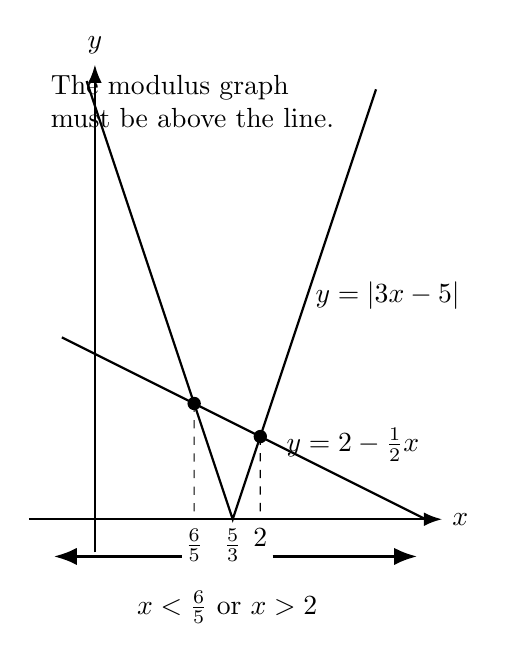
\begin{tikzpicture}[scale=1.05, >=Latex]
\draw[->, thick] (-0.8,0) -- (4.2,0) node[right] {$x$};
\draw[->, thick] (0,-0.4) -- (0,5.5) node[above] {$y$};
\draw[thick] (-0.1,5.3) -- (5/3,0) -- (3.4,5.2);
\node[right] at (2.55,2.7) {$y=|3x-5|$};
\draw[thick] (-0.4,2.2) -- (4,0);
\node[right] at (2.2,0.9) {$y=2-\frac12x$};
\coordinate (A) at (1.2,1.4);\coordinate (B) at (2,1);
\fill (A) circle (2.3pt);\fill (B) circle (2.3pt);
\draw[dashed] (A) -- (1.2,0);\draw[dashed] (B) -- (2,0);
\node[below] at (1.2,0) {$\frac65$};\node[below] at (2,0) {$2$};\node[below] at (5/3,0) {$\frac53$};
\draw[very thick, ->] (1.05,-0.45) -- (-0.5,-0.45);\draw[very thick, ->] (2.15,-0.45) -- (3.9,-0.45);
\node[below] at (1.6,-0.75) {$x<\frac65\ \text{or}\ x>2$};
\node[align=left, anchor=west] at (-0.65,5.05) {The modulus graph\\must be above the line.};
\end{tikzpicture}
\end{document}
